\documentclass[10pt]{article}
\usepackage[utf8]{inputenc}
\usepackage[T1]{fontenc}
\usepackage{graphicx}
\usepackage[export]{adjustbox}
\graphicspath{ {./images/} }
\usepackage{amsmath}
\usepackage{amsfonts}
\usepackage{amssymb}
\usepackage[version=4]{mhchem}
\usepackage{stmaryrd}

\title{\% \\ Portfolio Optimisation }

\author{}
\date{}


\begin{document}
\maketitle
Kannan Singaravelu, CQF

June 2023

\section*{Modern Portfolio Theory}
Modern portfolio theory also popularly called Mean-Variance Portfolio Theory (MVP) is a major breakthrough in finance. It is based on the premise that returns are normally distributed and by looking at mean and variance, we can essentially describe the distribution of end-of-period wealth.

The basic idea of this theory is to achieve diversification by constructing a portfolio for a minimal portfolio risk or maximal portfolio returns. Accordingly, the Efficient Frontier is a set of optimal portfolios in the risk-return spectrum, and portfolios located under the Efficient Frontier curve are considered sub-optimal.

This means that the portfolios on the frontier offered

\begin{itemize}
  \item Highest expected return for a given level of risk

  \item Lowest level of risk for a given level of expected returns

\end{itemize}

In essence, the investors' goal should be to select a level of risk that he/she is comfortable with and then find a portfolio that maximizes returns based on the selected risk level.

\subsection*{Import Libraries}
We'll import the required libraries that we'll use in this example.

\begin{center}
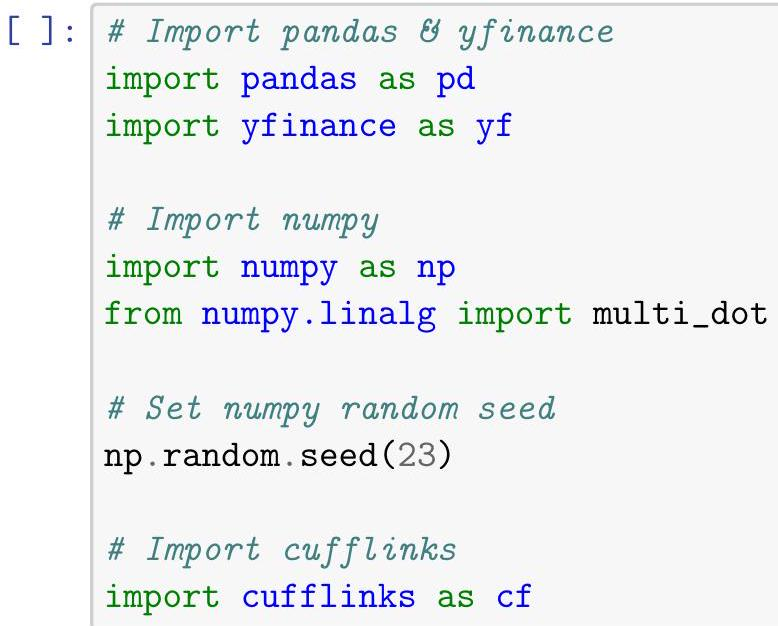
\includegraphics[max width=\textwidth]{2023_07_24_8a209382fdf398ddfaf7g-1}
\end{center}

\begin{center}
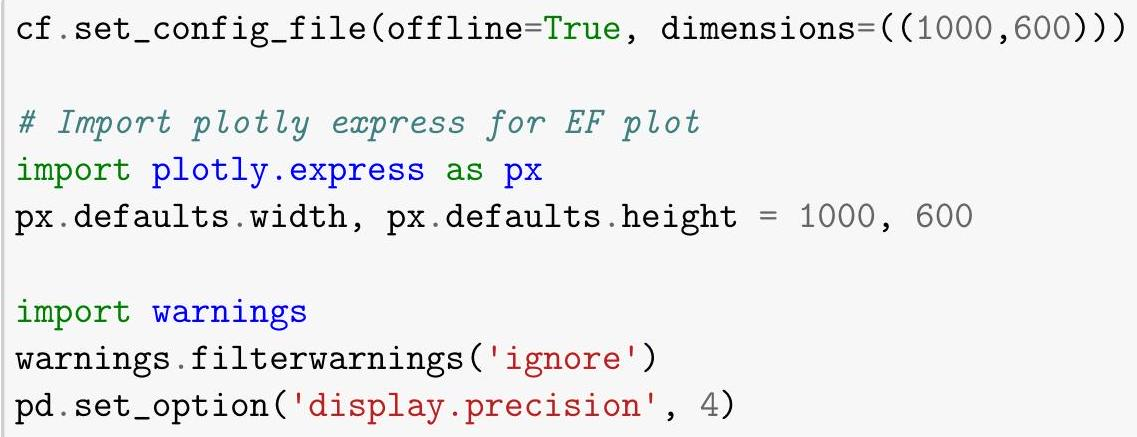
\includegraphics[max width=\textwidth]{2023_07_24_8a209382fdf398ddfaf7g-2}
\end{center}

\section*{$1.2 \quad$ Retrive Data}
We will retrieve price data from our list of stocks as before to build our portfolio

\begin{center}
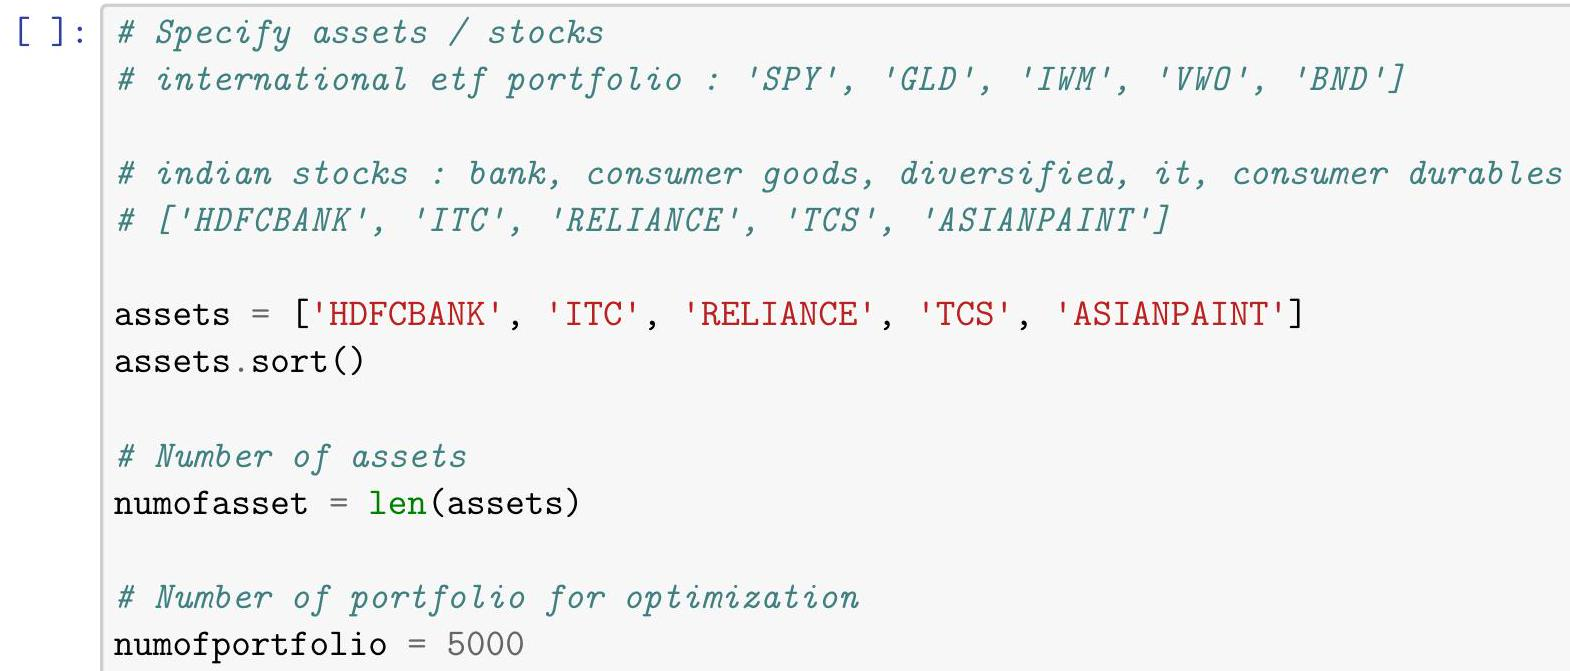
\includegraphics[max width=\textwidth]{2023_07_24_8a209382fdf398ddfaf7g-2(1)}
\end{center}

[ ]: \# Get yahoo tickers for indian stocks

\# yahooticker $=\left[x+{ }^{\prime} \cdot N S^{\prime}\right.$ for $x$ in assets $]$

\# Fetch / read data for multiple stocks at once

$\# d f=y f$. download (yahooticker, start='2015-01-01', end='2022-12-31', $\hookrightarrow$ progress $=$ False) $[$ 'Adj Close']

$\#$ df.columns $=$ assets

\# write data to file for future use

\# df.to\_csv('data/india\_stocks.csv')

\# Read from file

$\mathrm{df}=$ pd.read\_csv('data/india\_stocks.csv', index\_col=0, parse\_dates=True)

\# Display dataframe

df

\subsection*{Visualize Time Series}
[ ]: \# Plot price history

df ['2022':] .normalize(). iplot(kind='line')

[ ]: \# Dataframe of returns and volatility

returns $=$ df $\cdot$ pct\_change ()$\cdot$ dropna()

annual\_returns $=$ round (returns mean ()$* 260 * 100,2)$

annual\_stdev $=$ round $($ returns.std ()$* n p \cdot \operatorname{sqrt}(260) * 100,2)$

df $1=\operatorname{pd} \cdot$ DataFrame $(\{$

'Ann Ret': annual\_returns,

'Ann Vol': annual\_stdev

\})

[]$: \operatorname{df} 1$

[ ]: \# Plot annualized return and volatility

df1.iplot (

kind=' bar' ,

shared\_xaxes=True,

orientation $=' h$ '

)

\subsection*{Portfolio Composition}
[ ] : df1.reset\_index().iplot(

kind='pie' ,

labels = ' index',

values='Ann Ret',

textinfo='percent+label',

hole $=0.4$

)

\subsection*{Portfolio Statistics}
Consider a portfolio which is fully invested in risky assets. Let $w$ and $\mu$ be the vector of weights and mean returns of $n$ assets.

$$
w=\left(\begin{array}{c}
w_{1} \\
w_{2} \\
\vdots \\
w_{n}
\end{array}\right) ; \mu=\left(\begin{array}{c}
\mu_{1} \\
\mu_{2} \\
\vdots \\
\mu_{n}
\end{array}\right)
$$

where the $\sum_{i=1}^{n} w_{i}=1$

Expected Portfolio Return is then the dot product of the expected returns and their weights.

$$
\mu_{\pi}=w^{T} \cdot \mu
$$

which is also equivalent to the $\sum_{i=1}^{n} w_{i} \mu_{i}$

Expected Portfolio Variance is then the multidot product of weights and the covariance matrix.

$$
\sigma_{\pi}^{2}=w^{T} \cdot \Sigma \cdot w
$$

where, $\Sigma$ is the covariance matrix

$$
\Sigma=\left(\begin{array}{ccc}
\Sigma_{1,1} & \ldots & \Sigma_{1, n} \\
\vdots & \ddots & \vdots \\
\Sigma_{n, 1} & \ldots & \Sigma_{n, n}
\end{array}\right)
$$

\subsubsection*{Portfolio Simulation}
Now, we will implement a Monte Carlo simulation to generate random portfolio weights on a larger scale and calculate the expected portfolio return, variance and sharpe ratio for every simulated allocation. We will then identify the portfolio with a highest return for per unit of risk.

[ ]: def portfolio\_simulation(returns):

\# Initialize the lists

$\operatorname{rets}=[] ; \operatorname{vols}=[] ; \operatorname{wts}=[]$

\# Simulate 5,000 portfolios

for $i$ in range (numofportfolio):

\# Generate random weights

weights $=\mathrm{np} \cdot \mathrm{random} \cdot \mathrm{random}($ numofasset)

\# Set weights such that sum of weights equals 1

weights /=np.sum(weights)

\# Portfolio statistics

rets.append(weights. T @ np.array(returns.mean() * 260))

vols. append (np.sqrt (multi\_dot ([weights.T, returns.cov()*260, weights]))) wts. append (weights)

\# Create a dataframe for analysis

data $=\{$ port\_rets': rets, 'port\_vols': vols $\}$

for counter, symbol in enumerate(returns.columns.tolist ()) :

$\operatorname{data}[$ symbol+' weight' $]=[$ w[counter $]$ for $\mathrm{w}$ in wts $]$

portdf $=$ pd. DataFrame $($ data $)$

portdf ['sharpe\_ratio'] = portdf['port\_rets'] / portdf['port\_vols']

\subsubsection*{Maximum Sharpe Portfolio}
[ ]: \# Create a dataframe for analysis

temp = portfolio\_simulation (returns)

temp.head ()

[ ]: \# Get the max sharpe portfolio stats

temp.iloc[temp.sharpe\_ratio.idxmax()]

[ ]: \# Verify the above result

temp.describe ().T

\subsubsection*{Visulaize Simulated Portfolio}
[ ]: \# Plot simulated portfolio

fig $=$ px.scatter

temp, $\mathrm{x}=$ 'port\_vols', $\mathrm{y}=$ 'port\_rets', color='sharpe\_ratio',

labels=\{'port\_vols': 'Expected Volatility', 'port\_rets': 'Expected $\sqcup$

$\hookrightarrow$ Return', 'sharpe\_ratio': 'Sharpe Ratio'\},

title="Monte Carlo Simulated Portfolio"

). update\_traces (mode='markers ', $\operatorname{marker}=\operatorname{dict}\left(\operatorname{symbol}={ }^{\prime} \operatorname{cross}{ }^{\prime}\right)$ )

\# Plot max sharpe

fig.add\_scatter(

mode=' markers ',

$x=[$ temp. iloc [temp.sharpe\_ratio.idxmax ()] ['port\_vols']],

$\mathrm{y}=[$ temp. iloc[temp.sharpe\_ratio.idxmax ()] ['port\_rets']],

marker=dict (color='RoyalBlue', size=20, symbol='star' $)$,

name $=$ 'Max Sharpe'

). update(layout\_showlegend=False)

\# Show spikes

fig. update\_xaxes (showspikes=True)

fig. update\_yaxes (showspikes=True)

fig. show()

\subsection*{Efficient Frontier}
The Efficient Frontier is formed by a set of portfolios offering the highest expected portfolio return for a certain volatility or offering the lowest volatility for a certain level of expected returns.

Return objective:

$$
\operatorname{minimize}_{w_{1}, w_{2}, \ldots, w_{n}}^{2}\left(w_{1}, w_{2}, \ldots, w_{n}\right)
$$

subject to,

$$
E\left[R_{p}\right]=m
$$

Risk constraint:

$$
\underset{w_{1}, w_{2}, \ldots, w_{n}}{\operatorname{maximize}} E\left[R_{p}\left(w_{1}, w_{2}, \ldots, w_{n}\right)\right]
$$

subject to,

$$
\sigma_{p}^{2}\left(w_{1}, w_{2}, \ldots, w_{n}\right)=v^{2}
$$

where, $\sum_{i=1}^{n} w_{i}=1$ for the above objectives.

We can use numerical optimization to achieve this objective. The goal of optimization is to find the optimal value of the objective function by adjusting the target variables operating withing some boundary conditions and constraints.

\subsubsection*{Constrained Optimization}
Construction of optimal portfolios is a constrained optimization problem where we specify some boundary conditions and constraints. The objective function here is a function returning maximum sharpe ratio, minimum variance (volatility) and the target variables are portfolio weights. We will use the minimize function from scipy optimization module to achieve our objective.

[ ] : \# Import optimization module from scipy

\# sco.minimize?

import scipy.optimize as sco

\subsubsection*{Portfolio Statistics}
Let's subsume key statistics into a function which can be used for optimization exercise.

[ ] : def portfolio\_stats(weights):

weights $=\mathrm{np} \cdot \operatorname{array}($ weights $)$

port\_rets = weights.T (0 np.array(returns.mean()*260)

port\_vols $=n p . s q r t($ multi\_dot $([$ weights.T, returns.cov ()$* 260$, weights $]))$

return np.array([port\_rets, port\_vols, port\_rets/port\_vols])

\# Minimize the volatility

def min\_volatility(weights):

return portfolio\_stats(weights) [1]

\# Minimize the variance

def min\_variance(weights):

return portfolio\_stats(weights) [1] **2 \# Maximizing sharpe ratio

def max\_sharpe\_ratio(weights):

return -portfolio\_stats(weights) [2]

\subsubsection*{Efficient Frontier Portfolio}
For efficient frontier portfolios, we fix a target return and derive for objective function.

[ ]: \# Specify constraints, bounds and initial weights

cons $=(\{$ 'type': 'eq', 'fun': lambda $x: n p \cdot \operatorname{sum}(\mathrm{x})-1\})$

bnds = tuple $((0,1)$ for $\mathrm{x}$ in range(numofasset) $)$

initial\_wts $=$ numofasset $*[1 . /$ numofasset $]$

[ ]: \# Optimizing for maximum sharpe ratio

opt\_sharpe = sco.minimize(max\_sharpe\_ratio, initial\_wts, method='SLSQP', $\sqcup$

$\hookrightarrow$ bounds=bnds, constraints=cons)

\# Optimizing for minimum variance

opt\_var = sco.minimize(min\_variance, initial\_wts, method='SLSQP', bounds=bnds, $\sqcup$ $\hookrightarrow$ constraints=cons)

[ ] : opt\_sharpe

[ ] : opt\_var

[ ] : \# Efficient Frontier

targetrets $=\mathrm{np}$.linspace $(0.155,0.24,100)$

tvols $=[]$

for $\operatorname{tr}$ in targetrets:

ef\_cons $=$ (\{'type': 'eq', 'fun': lambda $x$ : portfolio\_stats $(x)[0]-\operatorname{tr}\}$, \{'type': 'eq', 'fun': lambda $x: n p \cdot \operatorname{sum}(\mathrm{x})-1\}$ )

opt\_ef = sco.minimize(min\_volatility, initial\_wts, method='SLSQP', $\sqcup$

$\hookrightarrow$ bounds=bnds, constraints=ef\_cons)

tvols. append (opt\_ef $\left[\right.$ 'fun ' $\left.^{\prime}\right]$ )

targetvols $=\mathrm{np} \cdot \operatorname{array}(\mathrm{tvols})$

[ ]: \# Create EF Dataframe for plotting

efport $=$ pd. DataFrame $(\{$

'targetrets' : np.around(100*targetrets, 2),

'targetvols': np.around (100*targetvols, 2),

'targetsharpe': np.around(targetrets/targetvols, 2) \})

efport.head()

[ ]: \# Plot efficient frontier portfolio

fig $=$ px.scatter (

efport, $\mathrm{x}=$ 'targetvols', $\mathrm{y}=$ 'targetrets', color='targetsharpe',

labels=\{'targetrets': 'Expected Return', 'targetvols': 'Expected $\sqcup$

$\hookrightarrow$ Volatility', 'targetsharpe': 'Sharpe Ratio'\},

title="Efficient Frontier Portfolio"

). update\_traces (mode='markers ', $\left.\operatorname{marker}=\operatorname{dict}\left(\operatorname{symbol}={ }^{\prime} \operatorname{cross}{ }^{\prime}\right)\right)$

\# Plot maximum sharpe portfolio

fig.add\_scatter(

mode=' markers ' ,

$\mathrm{x}=\left[100 *\right.$ portfolio\_stats (opt\_sharpe $\left.\left[\mathrm{x}^{\prime}\right]\right)$ ) $\left.[1]\right]$,

$\mathrm{y}=\left[100 *\right.$ portfolio\_stats (opt\_sharpe $\left.\left[\mathrm{x}^{\prime}\right]\right)$ ) $\left.[0]\right]$,

marker=dict (color='red', size=20, symbol='star'),

name $=$ 'Max Sharpe'

). update(layout\_showlegend=False)

\# Plot minimum variance portfolio

fig.add\_scatter(

mode=' markers ' ,

$\mathrm{x}=\left[100 *\right.$ portfolio\_stats $\left(\right.$ opt\_var $\left.\left.\left[\mathrm{x}^{\prime}\right]\right)[1]\right]$,

$\mathrm{y}=\left[100 *\right.$ portfolio\_stats (opt\_var $\left.\left.\left[\mathrm{x}^{\prime}\right]\right)[0]\right]$,

marker=dict (color='green', size=20, symbol='star' $)$,

name = 'Min Variance'

). update(layout\_showlegend=False)

\# Show spikes

fig.update\_xaxes (showspikes=True)

fig. update\_yaxes (showspikes=True)

fig.show()

\section*{References}
\begin{itemize}
  \item Numpy Linear Algebra

  \item Python Resources

  \item Scipy Optimization

  \item Styling Plotly Express Figures

  \item YFinance Documentation

\end{itemize}

June 2023, Certificate in Quantitative Finance.


\end{document}